\section{Introduction} \label{sec:intro}

% Johdatus aihepiiriin (ei liian laajasti, vaan relevantisti ja napakasti)
Before videocassette recorders became widely available for regular households, watching television was a very time-sensitive activity: if you wanted to see a TV program you had to watch it when it was broadcasted. When video recorders became affordable, they enabled people to record and watch TV programs whenever they wanted. Nowadays linear TV is losing even more of its foothold, as various video-on-demand services are gaining popularity. Recording storage is also moving away from the homes of viewers into the cloud servers of content providers.

Network personal video recorder (NPVR) is a type of service for recording broadcast TV programs for later viewing. Instead of storing recordings on the users local device, NPVR stores recordings on the content providers server. For every program listed in the Electronic program guide (EPG), a single recording is created and stored on the server. The users who record the same program will receive the same video from the server.

% Tutkimuskohteen esittely (MITÄ tämä työ tutkii? Kerro työstä/tutkimusaiheesta, ei omasta kirjoitusprosessistasi tai omasta kiinnostuksestasi.)
% Tutkimusongelma / -kysymykset (koko työsi sydän, jonka pitäisi näkyä ''punaisena lankana'' koko työn läpi)
% Tavoitteet (Käytä konkreettisesti sanaa ''tavoite'')
The NPVR recording start and end times are determined by the scheduling information given in the EPG. However, it is common that programs are not broadcasted exactly according to the EPG schedule. To make sure that the whole program is recorded, some margin is typically added on both ends of the recording. Thus NPVR recordings tend to have some non-program content at the beginning and end. The goal of this thesis is to study whether user viewing behaviour can be used in determining where the actual program content ends and where the closing credits begin in a NPVR recording.

% Tutkimuksen perustelu: ongelma tai aukko (aiemmassa tutkimuksessa on aukko, tai siitä nousee esiin kysymys, johon tässä etsitään vastausta)
I received this thesis topic from a company that is a NPVR service provider. There are a couple of motivations for closing credits detection. Firstly, less storage space is needed if the surplus contet after the closing credits is discarded. Secondly, if customers want to watch multiple episodes of a series in a row, it is very convenient for them if a link to the next episode is displayed during the closing credits, which requires knowing when the closing credits occur.

% Rajaus (Mitä tämä työ EI tutki)
% Menetelmä, aineisto, teoreettinen kehys (Esittele, MITEN em. aihetta tutkitaan)
User viewing behaviour might also be useful for detecting starting credits and advertisement breaks, but on this thesis I will focus on the closing credits detection to narrow down the topic. I will also restrict the examined recordings to TV series with multiple episodes and at least one hundred views per episode.

% Työn sisältö ja rakenne (Esittele, miten työn punainen lanka etenee, viittaukset työhön: ``ensin, sitten, seuraavaksi, luvussa 3'' jne.)
The thesis will consist of a case study of the closing credits detection based on user viewing behaviour, and a supporting literature review. The literature review section is divided in three parts. The first part discusses previous research on video content detection. The second part is about selecting a suitable model for determining the start time of the closing credits, based on the user viewing behaviour. The third part studies what are good methods for result evaluation and validation. The case study section first gives an overview on the data and ground truths. After that I will use the Python library Ruptures to detect the points where I suspect the closing credits occur. Finally I will evaluate and verify the results, and discuss the conclusions.

\section{Background} \label{sec:background}

\subsection{Video content detection} \label{subsec:detection}

\subsection{Signal change detection} \label{subsec:methods}

\subsection{Result evaluation and validation} \label{subsec:validation}

\section{Detecting end credits} \label{sec:casestudy}

\subsection{Baseline solution} \label{subsec:baseline}

The most straightforwad method for finding where the closing credits are, is is to have a human look at the recording. The accuracy of other methods can be evaluated by comparing their output to the ground truth obtained by this method.

Plotted in figure 1 is the time series of cumulative views per each second of an example recording. The red colored part of the plot is where the starting credits, advertisement break and closing credits of the program are. I checked the location of the aforementioned by looking at the recorded video. A steep increase in views can be seen in the plot whenever the actual program content begins, and correspondingly there is a steep decrease in views when the program content shifts into to advertisements or closing credits.

\begin{figure}[H]
    \centering
    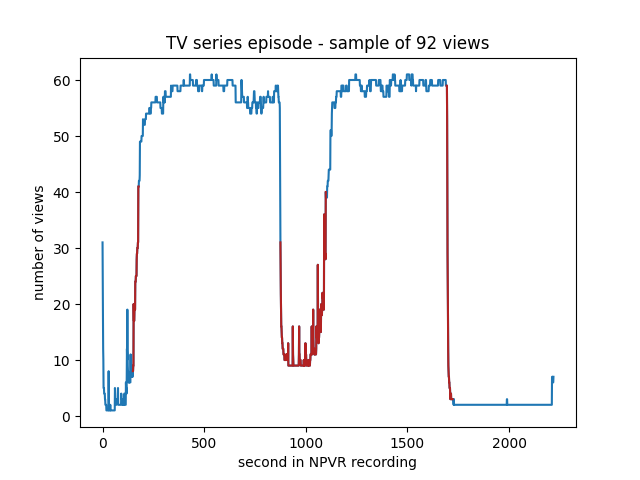
\includegraphics[width=1\textwidth]{../plots/episode.png}
    \caption{Example visualisation of user views count}
    \label{fig:intro_ads_outro}
    \end{figure}

\subsection{Detection with Ruptures library} \label{subsec:solution}


I will be using a Python library called Ruptures for the change point detection. Ruptures is based on the findings of a literature reviw conducted by \cite{truongSelectiveReviewOffline2020} which examines various methods for offline change point detection.

An example of Ruptures output is visualised on figure 2. The input data is the same as in figure 1. Red rectangles on the plot represent the actual location of the starting credits, advertisement break and closing credits, respectively. The vertical dashed lines indicate the change points determined by Rupture. They appear to be very close to the genuine change points at the edges of the red blocks.

I have collected the closing credits start and end time from 452 NPVR recordings by hand with a margin of error of ± 1 seconds. The cumulative views distribution similar as visualised in figure 1 can be calculated for each of the aforementioned recordings.

\begin{figure}[H]
\centering
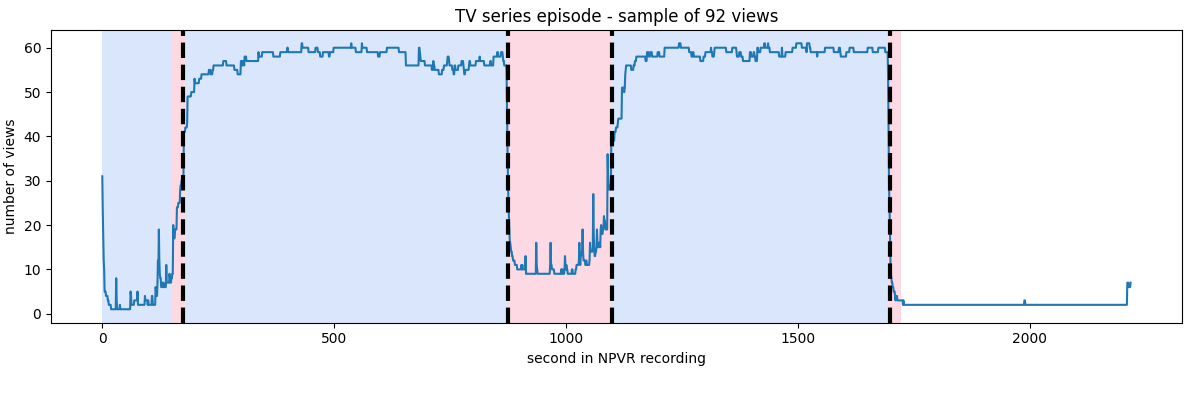
\includegraphics[width=1\textwidth]{../plots/episode-pen100.png}
\caption{Ruptures output for figure \ref{fig:intro_ads_outro} data}
\label{fig:ruptures_change_detection}
\end{figure}

\section{Results} \label{sec:results}

\section{Conclusions} \label{sec:conclusions}
